\chapter{Examples} \label{chap:examples}
results text...

\section{2D-problem 1: XOR function} \label{sec:dataset_xor}
XOR data...

\begin{figure}[H]
\centering
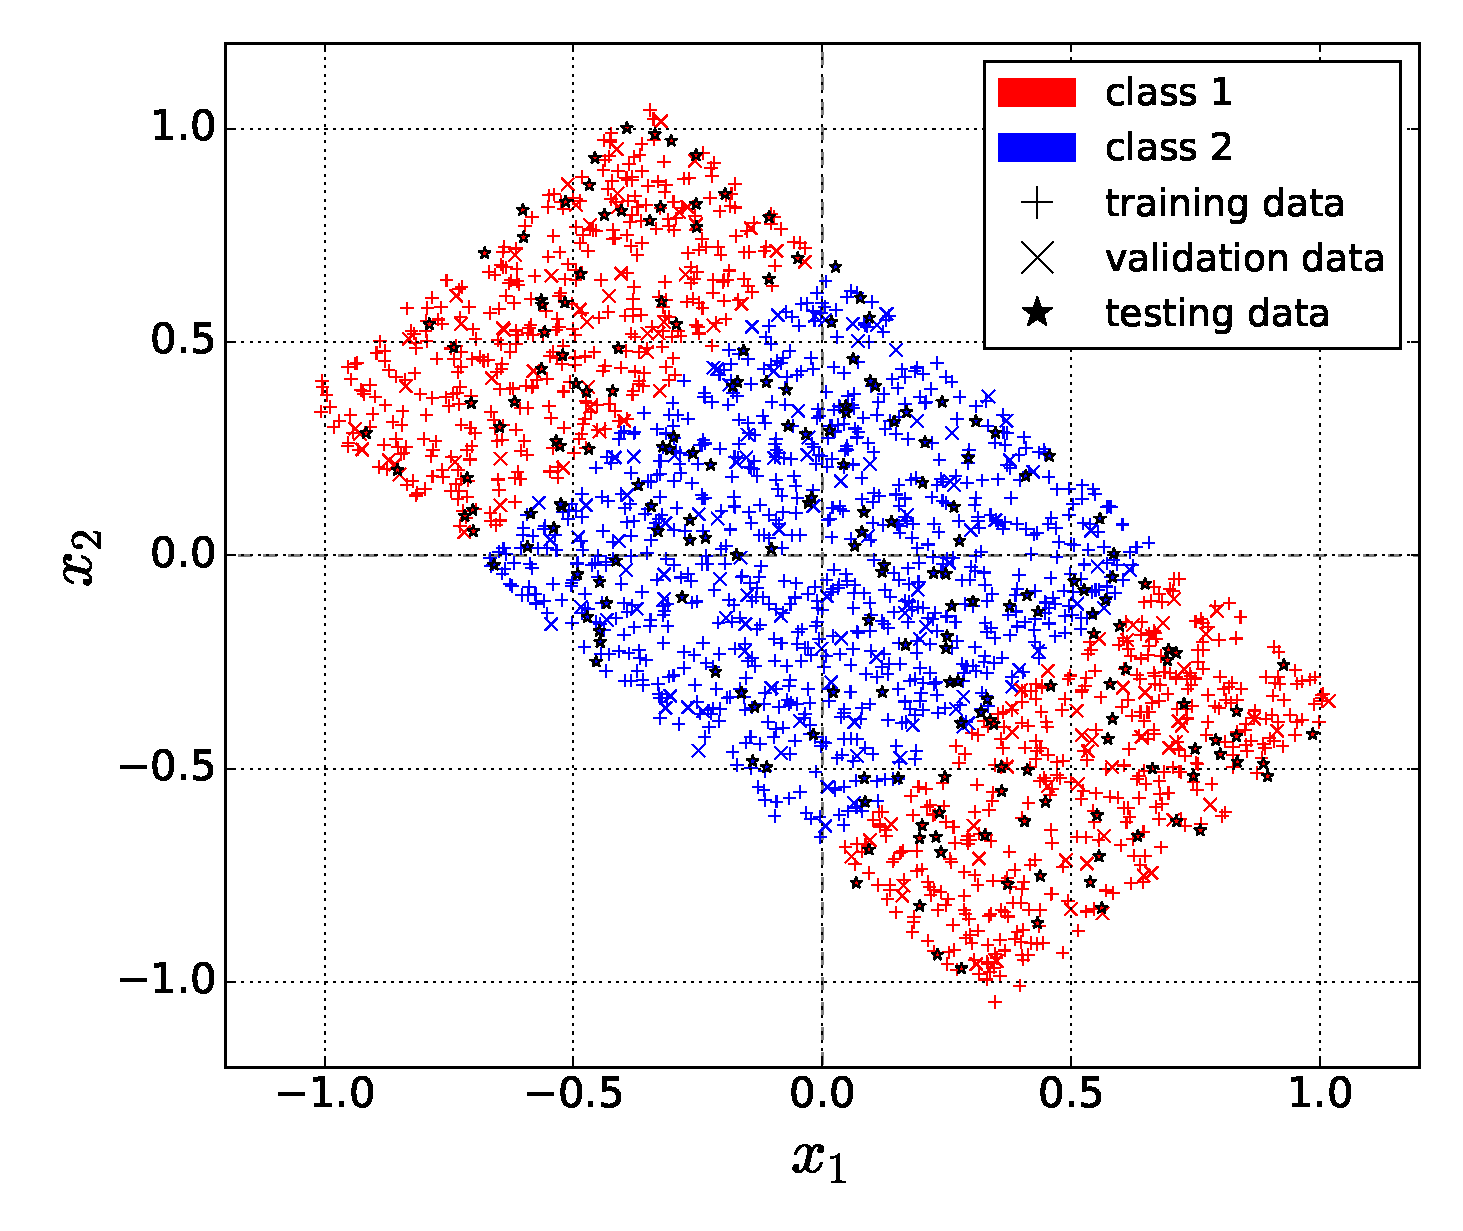
\includegraphics[width=\textwidth]{dataset_xor.eps}
\caption{The XOR dataset.}
\label{fig:examples:dataset_xor}
\end{figure}

\section{2D-problem 2: Unbalanced Features} \label{sec:dataset_unbfea}
Karnin data...

\begin{figure}[H]
\centering
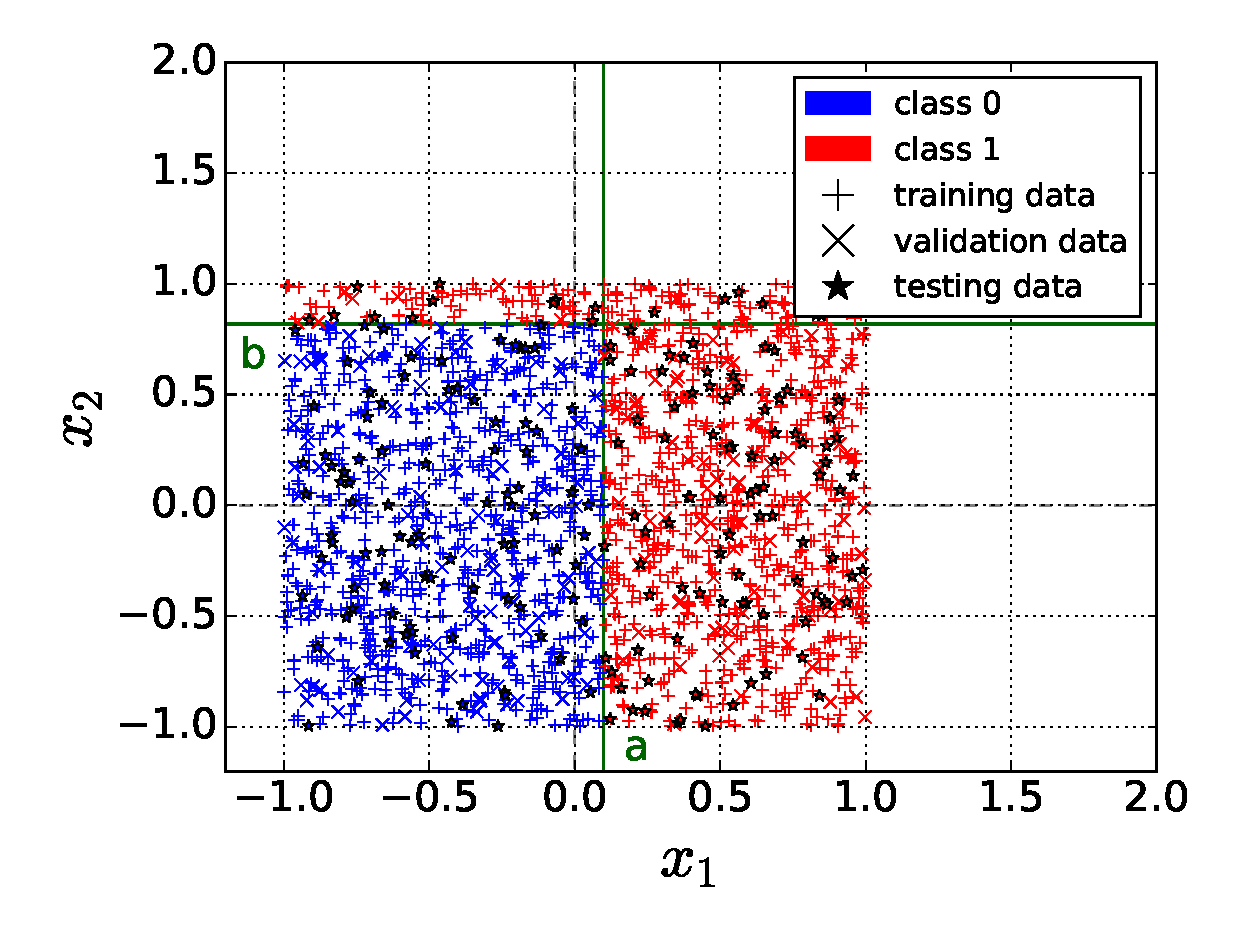
\includegraphics[width=\textwidth]{dataset_unbfea.eps}
\caption{The dataset with unbalanced features.}
\label{fig:examples:dataset_unbfea}
\end{figure}

\section{2D-problem 3: Rule Plus Exception} \label{sec:dataset_rpe}
RPE data...

\section{The Train Problem} \label{sec:dataset_train}
The Michalski's train problem...

\begin{figure}[H]
\centering
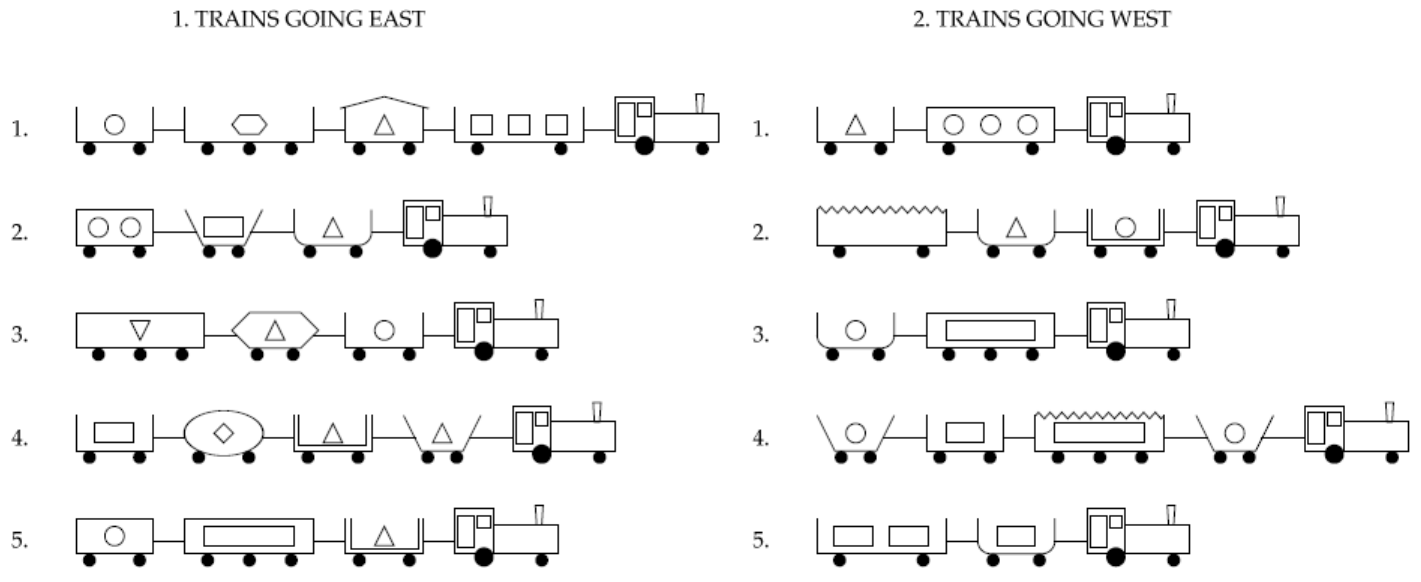
\includegraphics[width=\textwidth]{michalski_train_problem}
\caption{Michalski's train problem.}
\label{fig:examples:dataset_train}
\end{figure}

\section{Handwritten digits (MNIST)} \label{sec:dataset_mnist}
MNIST data... \citep{online:mnist}

\section{Phonemes (speech data)} \label{sec:dataset_phonemes}
PHONES data...
